%===================================================================================
% Chapter: Metodologia
%===================================================================================
\chapter{Experimentación y Resultados}\label{chapter:resultados}
%\addcontentsline{toc}{chapter}{Marco Teórico}
%===================================================================================

En este capítulo se detalla el proceso de validación del modelo propuesto. 

\section{Datos para la Validación del Modelo}
En el presente trabajo los datos provienen del Estudio en Lactantes Fase I/II para PCV7-TT (Instituto Finlay de Vacunas, 2019), cuyo principal objetivo era caracterizar la seguridad de VCN7-T y evaluar la no inferioridad de VCN7-T con respecto a Prevnar13® administrados en esquemas concomitante con las vacunas Va-Mengoc- BC® y Heberpenta® incluyendo lactantes de 2 a 3 meses de edad.

Se cuenta con datos de 240 sujetos divididos en dos grupos:
\begin{enumerate}
    \item Vacunados con VCN7-T
    \item Vacunados con Prevnar13®
\end{enumerate}

Para la validación del modelo nos centraremos en el grupo de sujetos vacunados con VCN7-T

\subsection{Limpieza de Datos}
Antes de trabajar con los datos fue realizado un proceso de limpieza de los mismos. 


\subsubsection{Análisis de Datos Faltantes}

Las Figuras \ref{fig:mdq} y \ref{fig:mdp} presentan el análisis de valores faltantes (nulos o vacíos) en las columnas de los conjuntos de datos para las vacunas VCN7-T (Figura \ref{fig:mdq}) y Prevnar13 (Figura \ref{fig:mdp}). 

\textbf{Descripción de las gráficas:}
\begin{itemize}
    \item \textbf{Eje Y:} Nombre de las columnas/variables del estudio
    \item \textbf{Eje X:} Cantidad de valores faltantes (expresada en conteo absoluto)
\end{itemize}

\begin{figure}[H]
    \centering
    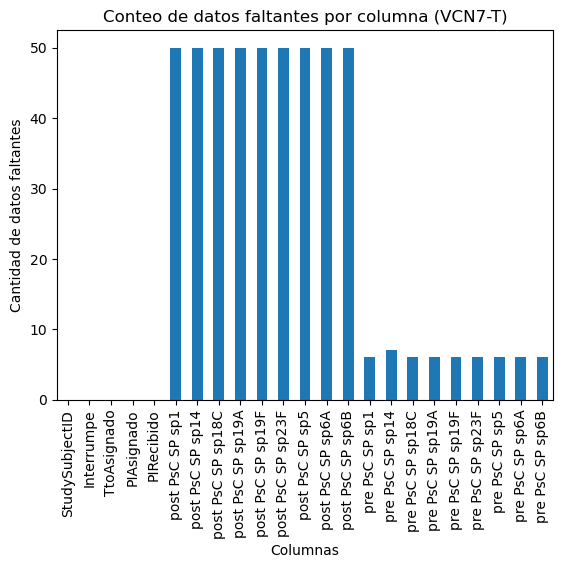
\includegraphics[width=0.7\textwidth]{Graphics/mdq.png}
    \caption{Distribución de valores faltantes por columna (VCN7-T)}
    \label{fig:mdq}
\end{figure}

\begin{figure}[H]
    \centering
    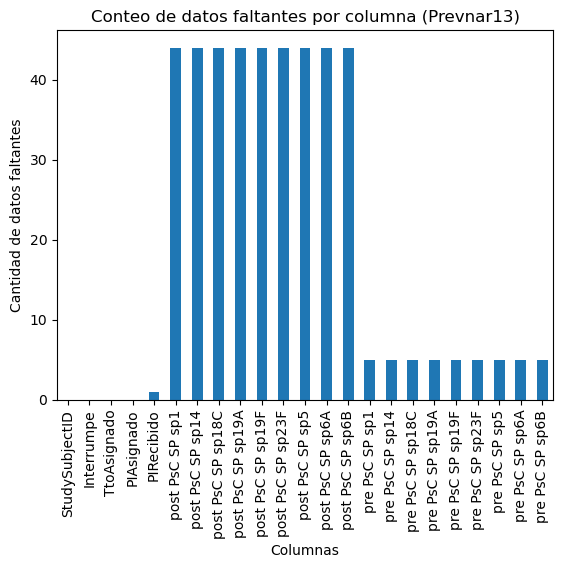
\includegraphics[width=0.7\textwidth]{Graphics/mdp.png}
    \caption{Distribución de valores faltantes por columna (Prevnar13)}
    \label{fig:mdp}
\end{figure}

La nomenclatura utilizada en los nombres de columna sigue este patrón:
\begin{itemize}
    \item \texttt{pre PsC SP [serotipo]:} Concentración de anticuerpos antes de la aplicación de la dosis de refuerzo (después de la dosis primaria) para un serotipo neumocócico específico
    \item \texttt{post PsC SP [serotipo]:} Concentración de anticuerpos después de la aplicación de la dosis de refuerzo para un serotipo neumocócico específico
    \item \texttt{[serotipo]:} Identificador del serotipo (e.g., sp1, sp14, sp19F, etc.)
\end{itemize}


Los altos valores en las columnas \texttt{post PsC SP [serotipo]} se consideran \textbf{no aleatorios} (MNAR - Missing Not At Random) y están directamente relacionados con el diseño del estudio, que incluyó dos esquemas de vacunación:

\begin{itemize}
    \item \textbf{Esquema (2p + 1):} Dos dosis primarias + refuerzo (mediciones post-refuerzo disponibles)
    \item \textbf{Esquema (3p + 0):} Tres dosis primarias sin refuerzo (mediciones post-refuerzo ausentes)
\end{itemize}

% Para la validación del modelo, se trabajó exclusivamente con los sujetos vacunados bajo el esquema (2p + 1), ya que:
% \begin{enumerate}
%     \item Presentan mediciones completas de anticuerpos post-vacunación
%     \item Permiten evaluar la respuesta inmune tras la dosis de refuerzo
%     \item Constituyen la cohorte con seguimiento completo
% \end{enumerate}

% \textbf{Justificación del enfoque:}
% La exclusión de sujetos con esquema (3p + 0) se basa en:
% \begin{itemize}
%     \item La imposibilidad de calcular la respuesta inmune completa sin mediciones post-vacunación
%     \item La necesidad de homogeneidad en el análisis de respuesta vacunal
%     \item La preservación de la validez interna del estudio
% \end{itemize}

En la investigación se asume que los sujetos con valores nulos en las columnas \texttt{post PsC SP [serotipo]} fueron vacunados siguiendo un esquema (3p + 0), sin embargo para la validación del modelo se trabajó en los sujetos vacunados siguiendo el esquema (2p + 1).

\subsubsection{Valores inconsistentes}
Durante el análisis de los datos, se detectaron valores atípicos con magnitudes aparentemente inconsistentes. Una inspección minuciosa reveló que dichos valores correspondían a cifras significativas expresadas con distinta notación decimal; en particular, mientras la mayoría de los datos estaban representados con tres cifras significativas correctamente posicionadas, algunos carecían del punto decimal, lo que implicaba una escala incorrecta. Para homogeneizar la representación, se aplicó una corrección que consiste en dividir por 1000 los valores afectados. Esta normalización facilitó una presentación más coherente y uniforme de los datos.

En las gráficas \ref{fig:sp1d}, \ref{fig:sp1}, \ref{fig:sp14d} y \ref{fig:sp14} (Gráficas de valores pre-refuerzo contra valores post-refuerzo) se muestra una comparación del estado de los datos antes y después de la corrección.


\begin{figure}[h]
    \centering
    % Primera fila
    \begin{minipage}{0.45\textwidth}
        \centering
        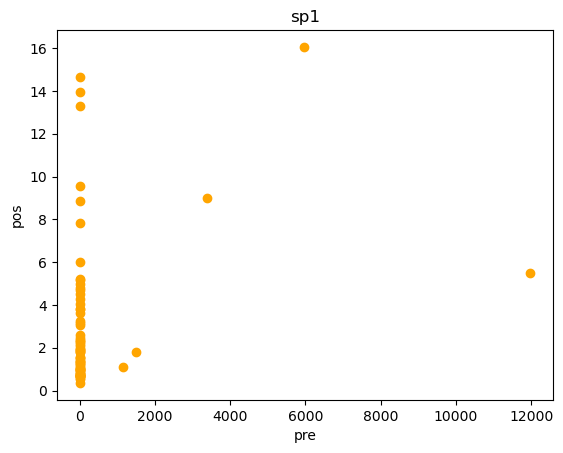
\includegraphics[width=\linewidth]{Graphics/sp1d.png}
        \caption{Serotipo 1 antes de la corrección}
        \label{fig:sp1d}
    \end{minipage}%
    \hfill
    \begin{minipage}{0.45\textwidth}
        \centering
        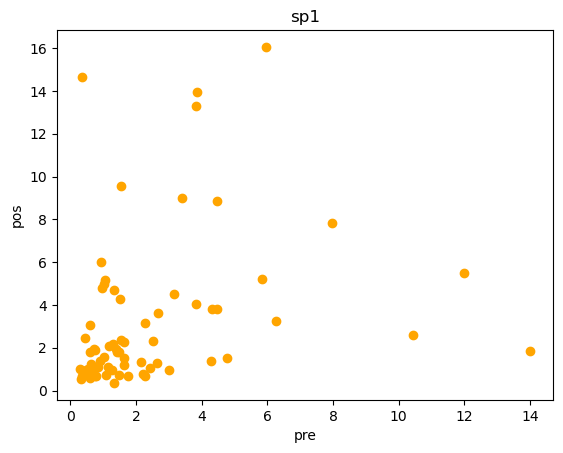
\includegraphics[width=\linewidth]{Graphics/sp1.png}
        \caption{Serotipo 1 después de la corrección}
        \label{fig:sp1}
    \end{minipage}

\end{figure}

\begin{figure}[H]
    \begin{minipage}{0.45\textwidth}
        \centering
        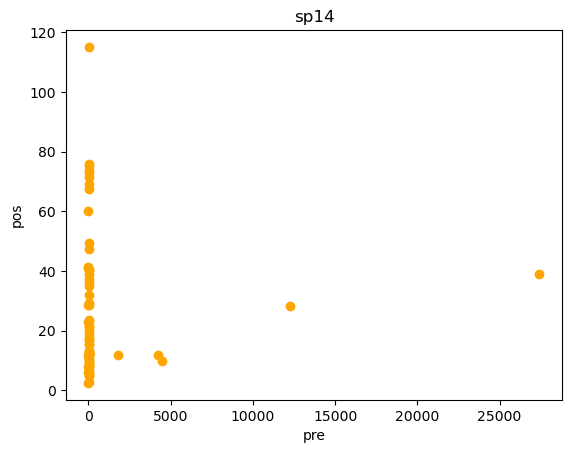
\includegraphics[width=\linewidth]{Graphics/sp14d.png}
        \caption{Serotipo 14 antes de la corrección}
        \label{fig:sp14d}
    \end{minipage}%
    \hfill
    \begin{minipage}{0.45\textwidth}
        \centering
        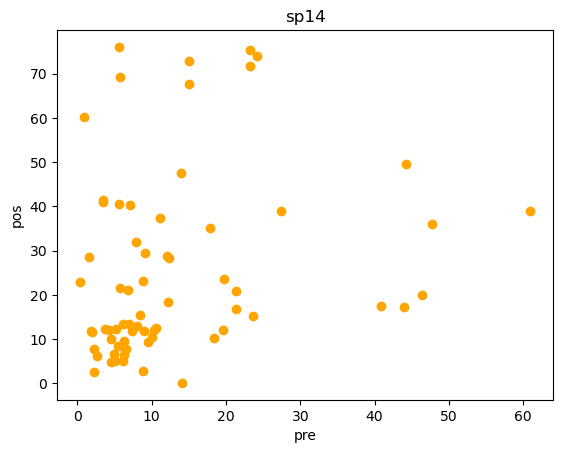
\includegraphics[width=\linewidth]{Graphics/sp14.png}
        \caption{Serotipo 14 después de la corrección}
        \label{fig:sp14}
    \end{minipage}
\end{figure}


\section{Entrenamiento}
Para el entrenamiento del modelo se tomó el 70\% de los datos. este proceso tiene como objetivo estimar los parámetros \texttt{plasma\_production\_factor} y \texttt{memory\_production\_factor}.

\subsection{Exploración del espacio de parámetros}

Para explorar el espacio de parámetros durante el proceso de entrenamiento se utilizó la metaheurística de Recocido Simulado (\textit{Simulated Annealing}). Este método permitió realizar una búsqueda estocástica evitando quedar atrapado en óptimos locales, gracias a su capacidad para aceptar temporalmente soluciones peores con una probabilidad controlada por un parámetro denominado temperatura.

El algoritmo comienza con una temperatura inicial 1.0 que permite explorar el espacio de soluciones, aceptando cambios incluso si empeoran la función objetivo. A medida que avanza el proceso, la temperatura decrece siguiendo un protocolo de enfriamiento, reduciendo gradualmente la probabilidad de aceptar soluciones peores.

\subsubsection{Soluciones vecinas:}
Estas se generan seleccionando aleatoriamente uno de los parámetros a estimar y añadiendole un ajuste $\delta$.

\subsubsection{Criteros de parada:}
\begin{itemize}
    \item \textbf{Enfriamiento del metal:} la temperatura es menor que \texttt{1e-3}.
    \item \textbf{Máximo de iteraciones:} se realizan más de 100 iteraciones.
\end{itemize}



\subsection{Función Objetivo}

La métrica utilizada como función objetivo durante el entrenamiento del modelo es la \textit{distancia de Chamfer} ($D_{\mathrm{Chamfer}}(S_1, S_2)$, donde \( S_1 \) y \( S_2 \) son los conjuntos de puntos simulados y reales), que es adecuada para comparar nubes de puntos, ya que evalúa la proximidad bidireccional entre cada punto de un conjunto y su vecino más cercano en el otro conjunto.

Minimizar la distancia de Chamfer durante el entrenamiento guía al modelo a generar salidas que se ajusten a los datos.


\section{Validación}
Para el proceso de validación se tomó el 30\% restante de los datos. Se generó una conjunto de la misma cantidad de puntos con los parámetros obtenidos en el proceso de entrenamiento y se calculó la distancia Chamfer para estos conjuntos. Los resultados obtenidos se muestran en la tabla \ref{tab:chamfer_serotipos}:

\begin{table}[h]
\centering
\caption{Distancia de Chamfer por Serotipo}
\begin{tabular}{|c|c|}
\hline
\textbf{Serotipo} & \textbf{Distancia Chamfer} \\
\hline
1   & 3.422  \\
14  & 26.348 \\
18C & 2.773  \\
19F & 4.443  \\
23F & 4.803  \\
5   & 3.241  \\
6B  & 8.539  \\
\hline
\end{tabular}
\label{tab:chamfer_serotipos}
\end{table}

\textbf{Gráficas de valores pre-refuerzo(post vacunación primaria) contra valores post-refuerzo}
\begin{itemize}
    \item Puntos naranjas: datos de validación.
    \item Puntos azules: salida del modelo.
\end{itemize}
\begin{figure}[h]
    \centering
    % Primera fila
    \begin{minipage}{0.45\textwidth}
        \centering
        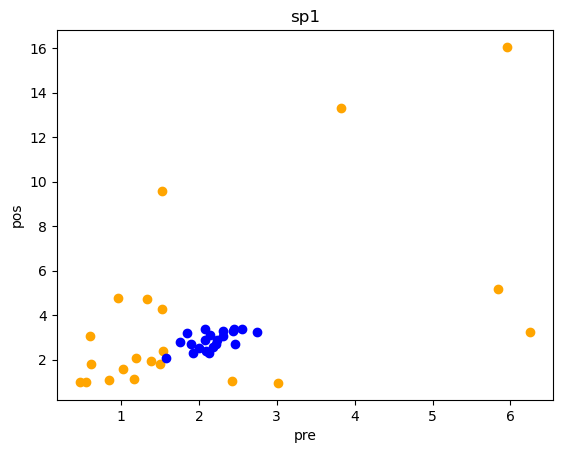
\includegraphics[width=\linewidth]{Graphics/sp1t.png}
        \caption{Serotipo 1}
        \label{fig:sp1t}
    \end{minipage}%
    \hfill
    \begin{minipage}{0.45\textwidth}
        \centering
        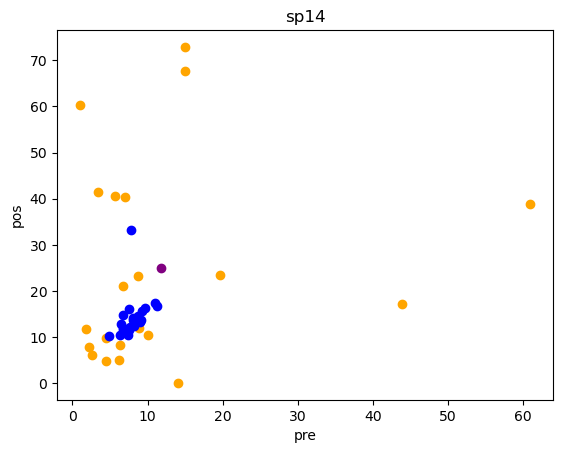
\includegraphics[width=\linewidth]{Graphics/sp14t.png}
        \caption{Serotipo 14}
        \label{fig:sp14t}
    \end{minipage}
\end{figure}
\begin{figure}
    
    \begin{minipage}{0.45\textwidth}
        \centering
        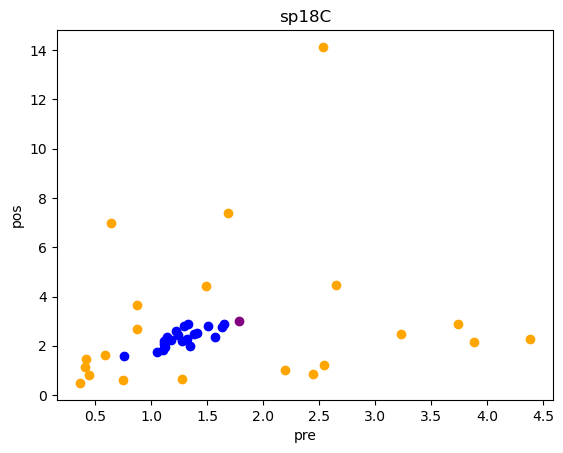
\includegraphics[width=\linewidth]{Graphics/sp18ct.png}
        \caption{Serotipo 18C}
        \label{fig:sp18ct}
    \end{minipage}
    \begin{minipage}{0.45\textwidth}
        \centering
        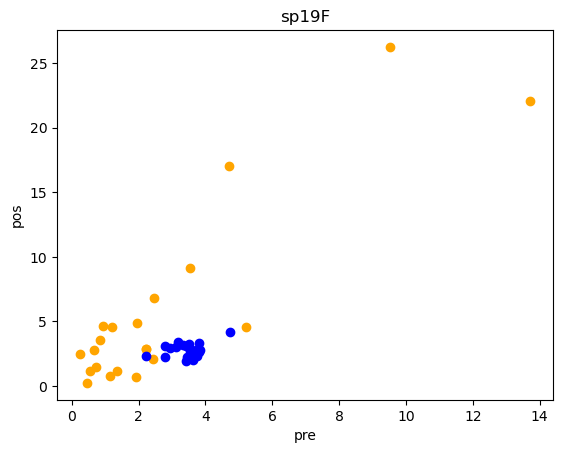
\includegraphics[width=\linewidth]{Graphics/sp19ft.png}
        \caption{Serotipo 19F}
        \label{fig:sp19ft}
    \end{minipage}
\end{figure}
\begin{figure}
    \begin{minipage}{0.45\textwidth}
        \centering
        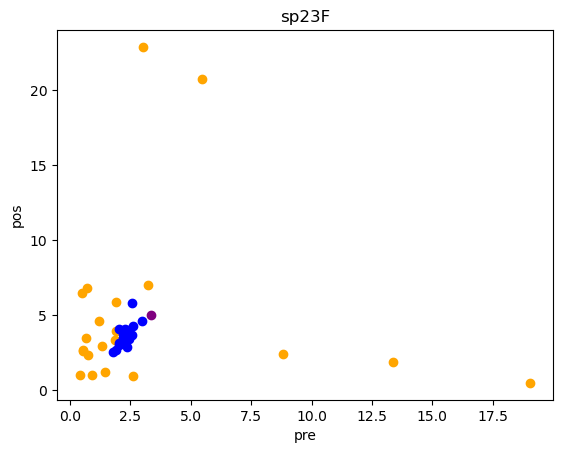
\includegraphics[width=\linewidth]{Graphics/sp23ft.png}
        \caption{Serotipo 23F}
        \label{fig:sp23ft}
    \end{minipage}
    \begin{minipage}{0.45\textwidth}
        \centering
        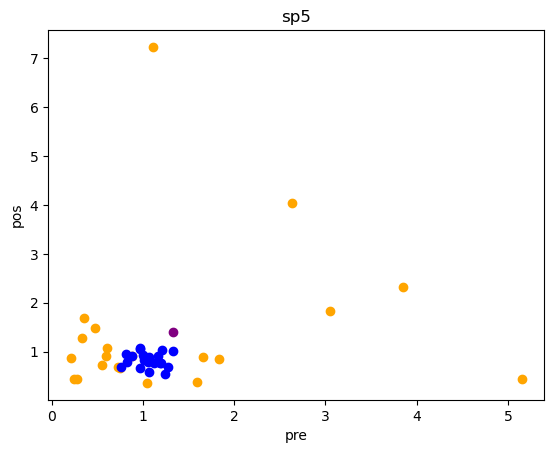
\includegraphics[width=\linewidth]{Graphics/sp5t.png}
        \caption{Serotipo 5}
        \label{fig:sp5t}
    \end{minipage}
\end{figure}
\begin{figure}
    \begin{minipage}{0.45\textwidth}
        \centering
        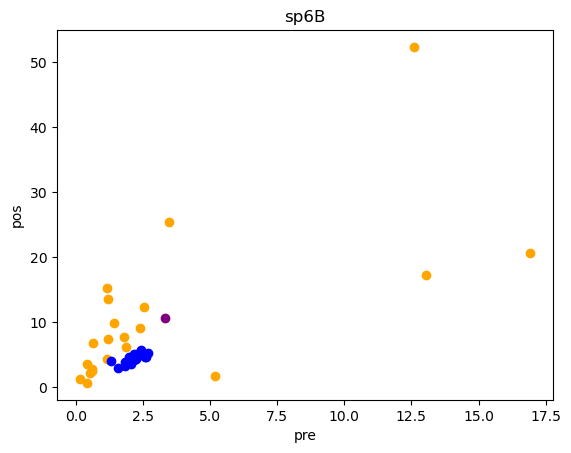
\includegraphics[width=\linewidth]{Graphics/sp6bt.png}
        \caption{Serotipo 6B}
        \label{fig:sp6bt}
    \end{minipage}

\end{figure}